\documentclass[a4paper, 12pt]{article}
%Paragraph jumps and indentation
\setlength{\parskip}{1.6em}
\setlength{\parindent}{1.25cm}
%Border
\usepackage[left=1in, right=1in, top=1in, bottom=1in]{geometry}
%Double spacing
\usepackage{setspace}
\usepackage{indentfirst}
\doublespacing
%Packages
\usepackage{amsmath}
\usepackage[dvipsnames]{xcolor}
\usepackage{mathtools}
\usepackage{amsfonts}
\usepackage{titlesec}
%Images
\usepackage{graphicx}
\graphicspath{ {./images/} }
\usepackage{wrapfig}
\usepackage{float}
%Tables
\usepackage{multirow}
\usepackage{array}
\usepackage{tabu}
\titleformat{\section}
{\normalfont\large\bfseries}{\thesection}{1em}{}
\titleformat{\subsection}
{\normalfont\large\bfseries}{\thesubsection}{1em}{}
%Equation numbering
\counterwithin{equation}{section}
\usepackage{hyperref}
\urlstyle{same}
\hypersetup{pdfborder=0 0 0}
\usepackage[font=small,labelfont=bf]{caption}

\begin{document}

\begin{titlepage}
\begin{center}
\vspace*{4cm}
{\huge\textbf{An inquiry about the uniqueness of the solution for the game of light off}}
\end{center}
\vspace{1cm}
\begin{flushright}
RQ:How many fundamentally different solutions are there to a game of light off.\\
Mathematics, Exam Session of 2025\\
% 2701 words
% inline math expression(not equation) 140
Word count:2841\\
\end{flushright}
\end{titlepage}

\tableofcontents
\clearpage

\section{Introduction}
In this essay we will be looking for a way to find the number of fundamentally unique solutions to a game of light off.
% 24

First, we need to understand the rule of the puzzle. The puzzle is played on a grid, where each square can either be on or off, like a light. Initially some of the squares are on and some are off. The player’s goal is to toggle all the squares off. To do so, the player can click one light, and all four (or less if it is on an edge or a corner) neighbor squares, along with itself, will be toggled.
% 81 105

The puzzle is quite interesting to analyze from a mathematical point of view because of its simple rules. The move can be modeled using the logic operator xor (exclusive or, written as ``$\oplus$", $a \oplus b =1$ when exactly one of $a$ and $b$ is true) or using addition under mod 2. The game can be easily made into a linear algebra problem of solving $XA = B$ for $X$, where $A$ is a constant and $B$ is a variable that we need to solve. 
% 71 176

The solutions depend on the initial states of the grid. Although there might be many different solutions, some of them are fundamentally the same. Our goal is to find out the number of fundamentally distinct solutions for a game that is solvable.
% 42 218

\clearpage
\section{Analysis}

\subsection{What counts as a unique solution}
\begin{wrapfigure}{r}{0.25\textwidth}
    \centering
    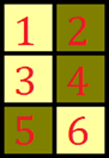
\includegraphics[width=0.15\textwidth]{img1.png}
    \caption{An example of a game, with each square labeled.}
\end{wrapfigure}

First, we need to define what counts as a unique solution. Let’s use the example on the right.
% 21 239 -3

The lights are numbered from 1 to 6 so it is easier to describe. One solution is to click 2 and click 4. Here is a detailed explanation of how the solution works. Clicking 2 switches 2 on, while also switch 4 on and 1 off. So now the lights that are on are light 2, 3, 4 and 6. Clicking 4 will switch 4 off, along with 2, 3 and 6, achieving the goal of switching every light off.
% 63 302

However, it is easy to see that clicking the two lights in different order will yield exactly the same effect, as the order of clicks does not matter. So we will consider two solutions that only differ by order of clicking equivalent. For example, we consider clicking 2 after 4 equivalent to clicking 4 after 2.
% 52 354

Another thing we may notice is clicking the same light twice cancels itself out. For example, if we click 1, the lights 1, 2 and 3 will toggle their states. If we click 1 again, the lights toggle states again to their original states. Thus, the solutions 2 4, 2 2 2 4, 2 3 4 3 ... are essentially the same. So we will consider all of them equivalent to the solution 2 4.
% 57 411

But not all solutions are equivalent after the above two transformation. For example, 3 6 is also a solution of the example game. However, we cannot convert it into 2 4 with the above two operations. Hence, we consider them different solutions.
% 38 449

\subsection{ Expressing the problem mathematically }
To find how many different solutions the example game has, we need a better way to represent a solution. As shown above, for all solutions that require one light to be clicked more than once, there is a equivalent solution where the light is clicked less times. So each light need to be clicked at most once. To represent a solution, we will simply number the lights row by row, and then list the number of time each light is clicked. For example, the solution of clicking 2 and 4 can be written as (0, 1, 0, 1, 0, 0). The length of the list is equal to the number of squares on the board.
% 102 551 +5

Using this notation, we can easily see there are exactly \(2^{m\times n}\) distinct actions, where $n$ and $m$ are the number of rows and columns, respectively. One way we can find the number of solutions is to try every action, and to count how many of those work. While this is possible to do, the calculation will take a lot of time,  and is infeasible for a large board even with the best computer.\footnote{The time complexity is used in computer science to indicates how the calculation time scale with data size. For this method, the time complexity is \(O(2^{n\times m})\), a very fast growing function.}
% 99 650 +1

The same notation can be used to express other things. Previously, we use it only to describe the steps used to solve a puzzle, but we can also use it to describe an action. An action will be defined as clicking some lights without necessarily solving the game. A solution is simply an action that result in an empty board after applied to the initial states.
% 65 715 +1

This allows us to do operations on actions. The sum of two actions is an action that has the same effect as doing both actions. To calculate the sum of two actions, we just need to add up the number of times a light is clicked, and then remove duplicate click. For example, to calculate (0, 1, 0, 1, 0, 0) + (0, 1, 1, 0, 1, 0), we first add up clicks of each light to get (0, 2, 1, 1, 1, 0). Then, since light 2 is clicked more than once, we subtract 2 from it, yielding the final answer of (0, 0, 1, 1, 1, 0). We will also define \textbf{0} as an action with no light clicked. 
% 92 807 +1

We can also find some properties. For example, if $A$, $B$ and $C$ are some actions, and \textbf{0} is the empty action, then the following hold:
% 21 828 +1
\vspace{-1.5cm}
\begin{singlespace}
\begin{itemize}
  \item \(A+B=B+A\)
  \item \((A+B)+C = A+(B+C)\)
  \item \(A+\textbf{0} = A\)
  \item \(A+A = \textbf{0}\)
\end{itemize}
\end{singlespace}

The first three properties follow from similar properties of addition. We just need to apply it to each light and then subtract 2 if needed. The \(4^{th}\) property comes from the fact that clicking a light twice has no effect. 
% 38 866 +1

Interestingly enough, the same data structure can also be used to describe the effect of an action, which is defined as the changes in states of lights resulted from an action. The value in the array now indicates if the corresponding light is toggled. Like before, flipping a light twice is equivalent to not flipping it as all. Addition will also work as before, with all the properties.
% 67 933 +1

We will also define function $f:X\mapsto B$ as a function that map an action to its effect. The function takes in an action ($X$) and yields the effect ($B$) of that action.
% 28 961

If the initial board state is $B$, and $f(X)=B$, then the effect of applying action $X$ is:
% 13 974 + 1
\[B+f(X)=B+B=\textbf{0}\]

Thus we can also view $X$ as the steps needed to solve a game with initial position $B$. After we find the function $f$, all we have to do is to find the number of unique solutions for $f(X)=B$, given $B$, to solve the problem.
% 42 1016 -2

First we can manually define the function for $X$, where all but one element in X is 0, that is, $X$ is an action that only click a single light. The function would be a map from those actions to their result. For example, with a board of 3 rows and 2 columns, $f((1, 0, 0, 0, 0, 0)) = (1, 1, 1, 0, 0, 0)$.
% 44 1060 +4

It should not be hard to see the function is lineal, that is, $f(X_1+X_2)=f(X_1)+f(X_2)$. Since every action can be expressed as a sum of actions that click only one light, to find $f(X)$, we can decompose $X$ into sum of those, and find the sum of the effects of those single light actions. For example, to calculate $f((0,1,0,1,0,0))$:
% 50 1110 +3
\[
\begin{split}
f((0,1,0,1,0,0)) & =f((0,1,0,0,0,0))+f((0,0,0,1,0,0))\\
& =(1,1,0,1,0,0)+(0,1,1,1,0,1)\\
& =(1,0,1,0,0,1)
\end{split}
\]

Previously, we just write actions and effects as a list. However, since the above calculation is very similar to vector multiplication, we can treat both actions and effects as a column vector.\footnote{However, for ease of reading, it will still appear as a list in text} Now to achieve the calculation above, we can construct a vector of vector, which we will call $M$, whose $i^{th}$ element is equal to $f(X)$, where $X$ is the action with only $i^{th}$ element 1. If we treat both $M$ and $X$ as vector, \(f(X) = M\cdot X\), where ``\(\cdot\)" denote inner product.\footnote{Inner product of vector \(A:(a_1, a_2, a_3,\ldots,a_n)\) and \(B:(b_1,b_2,b_3,\ldots,b_n)\) is equal to \(a_1b_1+a_2b_2+a_3b_3+\ldots+a_nb_n\)}\footnote{Note that multiplication was not defined before. So here we will define it to be the same as normal multiplication with integer, that is, $0\cdot A=0$ and $1\cdot A=A$.} However, since each element of $M$ is vector, we can also treat $M$ as a Matrix, which is the interpretation we will use from now on. $M$ is only dependent on the size of the game, not on the initial states. We shall denote $M$ for a game with $n$ rows $m$ columns as $M_{n, m}$. For example, to construct $M_{3,2}$:
% 168 1278 +3
\vspace{-1cm}
\begin{singlespace}
\begin{align*}
%0
f\left(\begin{pmatrix}1\\0\\0\\0\\0\\0\end{pmatrix}\right) =&
\begin{pmatrix}1\\1\\1\\0\\0\\0\end{pmatrix}&
%1
f\left(\begin{pmatrix}0\\1\\0\\0\\0\\0\end{pmatrix}\right) =&
\begin{pmatrix}1\\1\\0\\1\\0\\0\end{pmatrix}&
%2
f\left(\begin{pmatrix}0\\0\\1\\0\\0\\0\end{pmatrix}\right) =&
\begin{pmatrix}1\\0\\1\\1\\1\\0\end{pmatrix}\\
%3
f\left(\begin{pmatrix}0\\0\\0\\1\\0\\0\end{pmatrix}\right) =&
\begin{pmatrix}0\\1\\1\\1\\0\\1\end{pmatrix}&
%4
f\left(\begin{pmatrix}0\\0\\0\\0\\1\\0\end{pmatrix}\right) =&
\begin{pmatrix}0\\0\\1\\0\\1\\1\end{pmatrix}&
%5
f\left(\begin{pmatrix}0\\0\\0\\0\\0\\1\end{pmatrix}\right) =&
\begin{pmatrix}0\\0\\0\\1\\1\\1\end{pmatrix}
\end{align*}
, so % 1 1279
\begin{equation*}
M_{3,2}=\begin{pmatrix}
1&1&1&0&0&0\\
1&1&0&1&0&0\\
1&0&1&1&1&0\\
0&1&1&1&0&1\\
0&0&1&0&1&1\\
0&0&0&1&1&1
\end{pmatrix}
\end{equation*}
\end{singlespace}

Treating $X$, $B$ as vectors and $M$ as a matrix, the problem has become solving the equation $MX=B$. This is a common problem in linear algebra with many methods to solve it. However, here we are interested in the number of solutions. Usually, if the determinant of the matrix is non-zero, there is only one solution, otherwise there are either an infinite number of solutions, or none at all.
% 67 1346 -2

In this case, however, the variables are not real numbers like in normal system of linear equations, so the number of solutions for a certain case will always be finite due to the finite numbers of $X$. %And since a solution exists, the last possibility is also eliminated.
% 62 1408 -11

We are looking for the number of solutions to the equation $MX=B$, which is equivalent to finding the size of the solution set. We assume the equation is consistent (has at least one solution). Therefore, the solution set of $MX=B$ is merely a translation of the solution set equation $MX=0$ and must have the same size.\footnote{ Proof: Let $S$ be the set of all solutions to $MX=0$, $V$ is the solution set of $MX=B$, then if $X_1\in V$, for all $A\in S$, $M(X_1+A)=MX_1+MA=B+0=B$, so $X_1+A\in V$. Furthermore, if $MX_2=B$, $M(X_1+X_2)=MX_1+MX_2=0$, so $X_1+X_2\in S$. This means there is a injective function from $S$ to $V$ as well as from $V$ to $S$, hence they have the same size.} This further means that the number of solutions is the same for any solvable initial states provided the size of the board is the same. Our task has become to find the size of solution set $V$ of $MX=\textbf{0}$.
% 131 1539 +1
% Note_Cite

``The null space of $A$ is the subspace of $\mathbb{R}^n$ consisting of all solutions of the homogeneous equation  $Ax=\textbf{0}$"(Margalit, Dan, and Joseph Rabinoff. Subspaces), ``The nullity of a matrix $A$, written $nullity(A)$, is the dimension of the null space $Nul(A)$"(Margalit, Dan, and Joseph Rabinoff. The Rank Theorem). In our case, $V$ would, by definition, be the null space of $M$. Since we only deal with 0s and 1s, we can show the size of $V$ will be $2^{Nullity(M)}$.\footnote{If $B$ is a basis of the null space of $V$, then $B$ must a set of linear independent vector. That is to say if $B$ is a vector, $BX=0$ would only have one solution of $X=0$. $B$ is a basis also mean that every element in $V$ can be expressed as a lineal combination of $B$, and every linear combination of $B$ is in $V$. So $V$ is the set form from $BX$ for all vector $X$ with the same size as $B$ (which is equal to nullity of $M$) and is made up of 0 and 1. There are a total of $2^{Nullity(M)}$ possible value of $X$, and if $BX_1=BX_2$, $BX_1+BX_2=0=B(X_1+X_2)$, so $X_1+X_2=0$ and $X_1=X_2$. Hence each different $X$ correspond to a different element in $V$. So the size of $V$ is equal to the number of different $X$.}
% 164 1703

\subsection{Calculation of \texorpdfstring{$Nullity(M)$}{Nullity(M)}}
To find the nullity of $M$, we first need to be able to easily construct $M_{n, m}$. Each column is the change in board states after clicking a light, with one column for every light. Thus $M_{n, m}$ is a $mn$ by $mn$ matrix. To see things more clearly, we will cut M into $n^2$ block of $m$ by $m$. Using $M_{2, 3}$ as example:
% 52 1755
\begin{singlespace}
\begin{equation*}
M_{3,2}=
\left(
\begin{array}{c|c|c}
\begin{matrix}1&1\\1&1\end{matrix}&
\begin{matrix}1&0\\0&1\end{matrix}&
\begin{matrix}0&0\\0&0\end{matrix}\\\hline
\begin{matrix}1&0\\0&1\end{matrix}&
\begin{matrix}1&1\\1&1\end{matrix}&
\begin{matrix}1&0\\0&1\end{matrix}\\\hline
\begin{matrix}0&0\\0&0\end{matrix}&
\begin{matrix}1&0\\0&1\end{matrix}&
\begin{matrix}1&1\\1&1\end{matrix}
\end{array}
\right)
\end{equation*}
\end{singlespace}

By cutting the matrix like this, we can quickly find the light corresponding to a row or column. For example, the $4^{th}$ column is in the $1^{st}$ place in the $2^{nd}$ block, so it corresponds to clicking the light at $1^{st}$ column $2^{nd}$ row on the board. Each light clicked toggles its own states, as well as the one next to it in the same row (unless it is next to the edge). The result can be seen in the blocks on the main diagonal. All of them have the same value, and we will denote this small matrix $A_m$. The light clicked also toggle the one above or below it in the same column. So for each block on the main diagonal we had a block above and below it with only the diagonal 1s. This block we shall denote $E$. It is also known as the unit matrix.\footnote{A unit matrix has some useful properties we will used, such as for any square matrix $A$ with the same dimensions, $AE=EA=A$.}
% 161 1916

So now we can rewrite $M$ in block matrix form for easier calculation.
% 12 1928
\begin{singlespace}
\begin{equation*}
M=
\begin{pmatrix}
A&E&\textbf{0}&\hdots&\textbf{0}&\textbf{0}\\
E&A&E&\hdots&\textbf{0}&\textbf{0}\\
\textbf{0}&E&A&\hdots&\textbf{0}&\textbf{0}\\
\vdots&\vdots&\vdots&\ddots&\vdots&\vdots\\
\textbf{0}&\textbf{0}&\textbf{0}&\hdots&A&E\\
\textbf{0}&\textbf{0}&\textbf{0}&\hdots&E&A
\end{pmatrix}, \hspace{0.25cm}
Where\hspace{0.2cm} A =
\begin{pmatrix}
1&1&0&\hdots&0&0\\
1&1&1&\hdots&0&0\\
0&1&1&\hdots&0&0\\
\vdots&\vdots&\vdots&\ddots&\vdots&\vdots\\
0&0&0&\hdots&1&1\\
0&0&0&\hdots&1&1
\end{pmatrix}
\end{equation*}
\end{singlespace}

The nullity of $M$ is equal to the number of columns without pivots. ``A pivot is the first nonzero entry of a row of a matrix in row echelon form.”(Margalit, Dan, and Joseph Rabinoff. Row Reduction.) A matrix can be turned into row echelon form by repeatedly applying elementary row-operations (swapping two rows, multiplying a row by a non-zero number, and multiplying a row by a number and add it to another row) until it matches the following requirements:
% 72 2000
\vspace{-1.5cm}
\begin{singlespace}
\begin{enumerate}
  \item All zero rows are at the bottom.
  \item The first nonzero entry of a row is to the right of the first nonzero entry of the row above.
  \item Below the first nonzero entry of a row, all entries are zero.
\end{enumerate}
\end{singlespace}
\vspace{-1cm}
(Margalit, Dan, and Joseph Rabinoff. Row Reduction.)
% 39 2039

 It is possible to show the row-operations can also be done to square block matrix with slight adjustment, although it should be noted that multiplication would be with another matrix on the left instead of with a number.\footnote{It is easy to see how the first row-operation can be used in block matrix. The second operation require left multiply by a matrix with non-zero determinant. Since such a matrix can be converted to unit matrix through elementary row-operation, and elementary row-operation is equivalent to left multiplication by elementary matrix, left multiplication by such matrix is equivalent to left multiplication by elementary matrix after increasing the dimensions. For the third operation we can expand it to see it is equivalent to row-operation to multiple rows, and the row-operation can be further separate to elementary row-operation from multiple rows.} Using this we can do operations on M much easier. Using $M_{5, m}$ as an example (0 is omitted).
 % 152 2191

Starting with the original matrix.
\begin{singlespace}
\begin{equation*}
\begin{pmatrix}
A&E&&&\\
E&A&E&&\\
&E&A&E&\\
&&E&A&E\\
&&&E&A\\
\end{pmatrix}
\end{equation*}
\end{singlespace}
Swapping row 1 with row 2, row 3, row 4 and row 5.
\vspace{-0.5cm}
\begin{singlespace}
\begin{equation*}
\begin{pmatrix}
E&A&E&&\\
&E&A&E&\\
&&E&A&E\\
&&&E&A\\
A&E&&&\\
\end{pmatrix}
\end{equation*}
\end{singlespace}
Multiplying row 1 by $A$ and adding it to row 5.
\vspace{-0.5cm}
\begin{singlespace}
\begin{equation*}
\begin{pmatrix}
E&A&E&&\\
&E&A&E&\\
&&E&A&E\\
&&&E&A\\
&A^2+E&A&&&\\
\end{pmatrix}
\end{equation*}
\end{singlespace}
Multiplying row 2 by $(A^2 + E)$ and adding it to row 5.
\vspace{-0.5cm}
\begin{singlespace}
\begin{equation*}
\begin{pmatrix}
E&A&E&&\\
&E&A&E&\\
&&E&A&E\\
&&&E&A\\
&&A^3&A^2+E&\\
\end{pmatrix}
\end{equation*}
\end{singlespace}
Multiplying row 3 by $(A^3)$ and adding it to row 5 (Note that $A+A=0$ since they cancel out with our definition of addition).
\vspace{-0.5cm}
\begin{singlespace}
\begin{equation*}
\begin{pmatrix}
E&A&E&&\\
&E&A&E&\\
&&E&A&E\\
&&&E&A\\
&&&A^4+A^2+E&A^3\\
\end{pmatrix}
\end{equation*}
\end{singlespace}
Multiplying row 4 by $(A^4+A^2 + E)$ and adding it to row 5.
\vspace{-0.5cm}
\begin{singlespace}
\begin{equation*}
\begin{pmatrix}
E&A&E&&\\
&E&A&E&\\
&&E&A&E\\
&&&E&A\\
&&&&A^5+A\\
\end{pmatrix}
\end{equation*}
\end{singlespace}
% 56 2247

Note that the first four rows already meet the requirement for row echelon form. Furthermore, the first four columns all have pivot element. This means all the columns without pivots would be in the bottom right matrix. Hence, $Nullity(M) = Nullity(A^5+A)$.
% 38 2285

Now we shall find the matrix on the bottom right for any $n$. After the initial row swapping, the bottom row always starts with $A$ and $E$, followed by 0s. We then repeat the process of eliminating the first non-zero element of the bottom row. Let $B_1$ be the first non-zero element on the bottom row originally (after swapping). $B_2$ will be the first non-zero element on the bottom row after one operation and so on. It can be noted that $B_i$ will be the first non-zero element located in column $i$. Let $C_i$ be the element that follows $B_i$. If $i<n$, the next operation will remove $B_i$. Row $i$ column $i$ is always equal to $E$, and row $i$ column $i+1$ equal $A$. To remove $B_i$, we can left multiply row $i$ by $B_i$ and add it to the bottom row. This will cancel out $B_i$, so $B_{i+1} = C_i + AB_i$, and $C_{i+1}$, if it exists, is equal to $B_i$.
% 134 2419
\begin{singlespace}
\begin{align*}
\begin{pmatrix}
E&A&E&&\\
&E&A&E&\\
&&E&A&E\\
&&&E&A\\
&B_{i}&C_{i}&&\\
\end{pmatrix}\overset{r_n+B_ir_i}{\longrightarrow}&
\begin{pmatrix}
E&A&E&&\\
&E&A&E&\\
&&E&A&E\\
&&&E&A\\
&B_{i}+B_{i}E&C_{i}+B_{i}A&B_{i}E&\\
\end{pmatrix}\\=&
\begin{pmatrix}
E&A&E&&\\
&E&A&E&\\
&&E&A&E\\
&&&E&A\\
&&C_{i}+B_{i}A&B_{i}&\\
\end{pmatrix}
\end{align*}
\end{singlespace}

Hence, for all $2<i\leq n$, $C_i = B_{i-1}$, so $B_i=C_{i-1}+AB_{i-1}=B_{i-2}+AB_{i-1}$. With $B_1 = A$ and $B_2=A^2+E$. Using this formula, we can find $B_n$ based on $n$ and $A$. Since $A$ can easily be constructed with $m$, we can then calculate $B_n$ for any $m, n>0$. The number of solutions would then be two to the power of Nullity of $B_n$.
% 41 2460

\subsection{Result}
Using all the formula above, I made a simple computer program to calculate the nullity of $M$ for all $0\leq m, n<10$,\footnote{While one will not encounter game with 0 rows or columns, it is listed here for easier observation of pattern. A game with 0 rows or columns will have only one solution of doing nothing and $\log_2(1) = 0$} listed in the table below. As proven in the essay, the number so solutions is simply $2^{nullity(M)}$, also listed below.
% 71 2531
\begin{singlespace}
\begin{samepage}
\[
Nullity(M)\]
\[
\begin{array}{c|cccccccccc}
{}_n\backslash{}^m&0&1&2&3&4&5&6&7&8&9\\\hline
0&0&0&0&0&0&0&0&0&0&0\\
1&0&0&1&0&0&1&0&0&1&0\\
2&0&1&0&2&0&1&0&2&0&1\\
3&0&0&2&0&0&3&0&0&2&0\\
4&0&0&0&0&4&0&0&0&0&4\\
5&0&1&1&3&0&2&0&4&1&1\\
6&0&0&0&0&0&0&0&0&6&0\\
7&0&0&2&0&0&4&0&0&2&0\\
8&0&1&0&2&0&1&6&2&0&1\\
9&0&0&1&0&4&1&0&0&1&8
\end{array}
\]
\end{samepage}
\vspace{1cm}
\begin{samepage}
\[
Number\hspace{0.2cm}of\hspace{0.2cm}solutions\]
\[
\begin{array}{c|cccccccccc}
{}_n\backslash{}^m&0&1&2&3&4&5&6&7&8&9\\\hline
0&1&1&1&1&1&1&1&1&1&1\\
1&1&1&2&1&1&2&1&1&2&1\\
2&1&2&1&4&1&2&1&4&1&2\\
3&1&1&4&1&1&8&1&1&4&1\\
4&1&1&1&1&16&1&1&1&1&16\\
5&1&2&2&8&1&4&1&16&2&2\\
6&1&1&1&1&1&1&1&1&64&1\\
7&1&1&4&1&1&16&1&1&4&1\\
8&1&2&1&4&1&2&64&4&1&2\\
9&1&1&2&1&16&2&1&1&2&256
\end{array}
\]
\end{samepage}
\end{singlespace}

\clearpage
\section{Conclusion}
Using some linear algebra, we have successfully found a way to calculate the number of possible solutions to a game of light off played on an $n$ by $m$ board. While the method might seem somewhat complicated for a game with such a simple game, that seem to be a common trend in some area of mathematics. The method explored here can be used to calculate the result in polynomial time,\footnote{ Matrix multiplication has time complexity of $O(m^3)$ without optimization for square matrix of dimensions $m\times m$. The calculation of $B_n$ require time complexity $O(nm^3)$. The calculation of nullity without optimization requires time complexity of $m^2$. Adding everything together, the total time complexity of $O(nm^3)$.} so the answer can be quickly calculated with a normal computer for $m,n<50$. However, I believe there might be a faster way to do so. It is possible to prove that the nullity of $M_{n,i}$ is periodic. It would be a very interesting problem to study the pattern in more detail, but that is beyond the scope for this essay.
% 165 2696

\clearpage
\section{Work cited}
\begin{description}

% prehaps unused
% \item Margalit, Dan, and Joseph Rabinoff. Basis and Dimension. Georgia Institute of Technology, 17 Sept. 2022, https://math.libretexts.org/@go/page/70192. 

% defo used
\item Margalit, Dan, and Joseph Rabinoff. Row Reduction. Georgia Institute of Technology, 17 Sept. 2022, https://math.libretexts.org/@go/page/70183. 

% include observation that could help with the "Note_cite"
% \item Margalit, Dan, and Joseph Rabinoff. Solution Sets. Georgia Institute of Technology, 17 Sept. 2022, https://math.libretexts.org/@go/page/70189. 

% used
\item Margalit, Dan, and Joseph Rabinoff. Subspaces. Georgia Institute of Technology, 17 Sept. 2022, https://math.libretexts.org/@go/page/70191. 

% used
\item Margalit, Dan, and Joseph Rabinoff. The Rank Theorem. Georgia Institute of Technology, 3 Apr. 2022, https://math.libretexts.org/@go/page/70193. 

\end{description}

\end{document}